\documentclass[a4paper,12pt]{article}
\usepackage[utf8]{inputenc}
\usepackage[T2A]{fontenc}
\usepackage[russian,english]{babel}
\usepackage[pdftex]{graphics}
\DeclareGraphicsExtensions{.pdf,.png,.jpg}
\graphicspath{{pictures/}}
\begin{document}
\begin{center}
Санкт-Петербургский государственный политехнический университет
\\Кафедра компьютерных систем и программных технологий
\end{center}
\vspace*{10em plus .6em minus .5em}

\begin{center}
{\LARGEТелекоммуникационные технологии
\\Лабораторная работа №3
\\Линейная фильтрация}
\end{center}

\vspace*{5em plus .6em minus .5em}
\begin{flushright}
Выполнил:\\студент гр.33501/4\\Курякин Д. А.\\Проверила:\\Богач Н.В.
\end{flushright}

\vspace*{15em plus .6em minus .5em}
\begin{center}
{\smallСанкт-Петербург
\\2018}
\end{center}
\pagestyle{empty}
\newpage
\pagestyle{plain}

\section{Цель}

Изучить воздействие ФНЧ на тестовый сигнал с шумом.

\section{Постановка задачи}

Сгенерировать гармонический сигнал с шумом и синтезировать ФНЧ. Получить сигнал во временной и частотной областях до и после фильтрации. Сделать выводы о воздействии ФНЧ на спектр сигнала.

\section{Теоретическое обоснование}

Фильтр в электронике -- устройство для выделения желательных компонентов спектра электрического сигнала и/или подавления нежелательных.

Фильтры бывают:
\begin{itemize}
 \item Аналоговые используются с аналоговыми или непрерывными сигналами.
 \item Цифровые  используются с дискретными сигналами.
 \item Пассивные -- электронный фильтр, состоящий только из пассивных компонентов, таких как, к примеру, конденсаторы и резисторы. Пассивные фильтры не требуют никакого источника энергии для своего функционирования.
 \item Активные -- это один из видов аналоговых электронных фильтров, в котором присутствует один или несколько активных компонентов, к примеру, транзистор или операционный усилитель. 
 \item Линейные -- динамическая система, применяющая некий линейный оператор ко входному сигналу для выделения или подавления определённых частот сигнала и других функций по обработке входного сигнала.
 \item Нелинейные -- устройство для обработки сигналов, выход которого не является линейным оператором от входного сигнала.
 \item Рекурсивный фильтр (БИХ-фильтр) -- линейный электронный фильтр, использующий один или более своих выходов в качестве входа, то есть образующий обратную связь. Такие фильтры могут быть как аналоговыми, так и цифровыми.
 \item Нерекурсивный фильтр (КИХ-фильтр) -  один из видов линейных цифровых фильтров, характерной особенностью которого является ограниченность по времени его импульсной характеристики (с какого-то момента времени она становится точно равной нулю). Такой фильтр называют ещё нерекурсивным из-за отсутствия обратной связи.
\end{itemize}

Среди множества рекурсивных фильтров отдельно выделяют следующие фильтры
\begin{itemize}
	\item Фильтры Чебышёва -- один из типов линейных аналоговых или цифровых фильтров, отличительной особенностью которого является более крутой спад амплитудно-частотной характеристики (АЧХ) и существенные пульсации амплитудно-частотной характеристики на частотах полос пропускания (фильтр Чебышёва I рода) и подавления (фильтр Чебышёва II рода), чем у фильтров других типов.
	\item Фильтры Бесселя -- в электронике и обработке сигналов один из наиболее распространённых типов линейных фильтров, отличительной особенностью которого является максимально гладкая групповая задержка (линейная фазо-частотная характеристика). Фильтры Бесселя чаще всего используют для аудио-кроссоверов. Их групповая задержка практически не изменяется по частотам полосы пропускания, вследствие чего форма фильтруемого сигнала на выходе такого фильтра в полосе пропускания сохраняется практически неизменной.
	\item Фильтры Баттерворта -- один из типов электронных фильтров. Фильтры этого класса отличаются от других методом проектирования. Фильтр Баттерворта проектируется так, чтобы его амплитудно-частотная характеристика была максимально гладкой на частотах полосы пропускания.
	\item Эллиптические фильтры --  электронный фильтр, характерной особенностью которого являются пульсации амплитудно-частотной характеристики как в полосе пропускания, так и полосе подавления. Величина пульсаций в каждой из полос независима друг от друга. Другой отличительной особенностью такого фильтра является очень крутой спад амплитудной характеристики, поэтому с помощью этого фильтра можно достигать более эффективного разделения частот, чем с помощью других линейных фильтров. Если пульсации в полосе подавления равны нулю, то эллиптический фильтр становится фильтром Чебышёва I рода. Если пульсации равны нулю в полосе пропускания, то фильтр становится фильтром Чебышёва II рода. Если же пульсации отсутствуют на всей амплитудной характеристике, то фильтр становится фильтром Баттерворта.
\end{itemize}

По тому, какие частоты фильтром пропускаются (задерживаются), фильтры подразделяются на
\begin{itemize}
	\item фильтры нижних частот -  электронный или любой другой фильтр, эффективно пропускающий частотный спектр сигнала ниже некоторой частоты (частоты среза) и подавляющий частоты сигнала выше этой частоты.;
	\item фильтры верхних частот -  электронный или любой другой фильтр, пропускающий высокие частоты входного сигнала, при этом подавляя частоты сигнала ниже частоты среза.;
	\item полосно-пропускающие фильтры -  фильтр, который пропускает частоты, находящиеся в некоторой полосе частот. Полосовой фильтр — линейная система и может быть представлен в виде последовательности, состоящей из фильтра нижних частот и фильтра верхних частот.;
	\item полосно-задерживающие фильтры -  электронный или любой другой фильтр, не пропускающий колебания некоторой определённой полосы частот, и пропускающий колебания с частотами, выходящими за пределы этой полосы.;
	\item фазовые фильтры - электронный или любой другой фильтр, пропускающий все частоты сигнала с равным усилением, однако изменяющий фазу сигнала..
\end{itemize}
\newpage

\section{Ход работы}

Сгенерируем гармонический сигнал
\center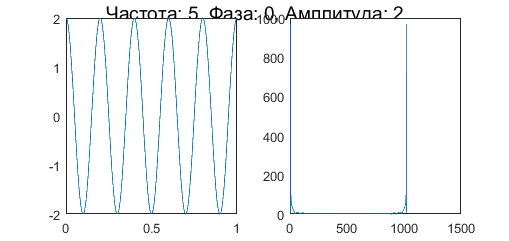
\includegraphics{pictures/sig.png} \\ Рис.1 Сигнал


Добавим к нему шум
\center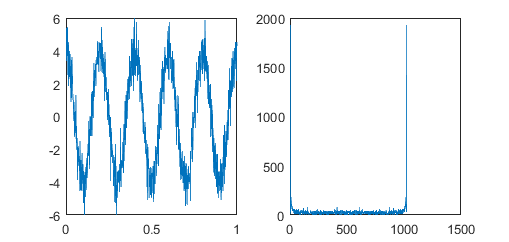
\includegraphics{pictures/shum.png} \\ Рис.3 Зашумленный сигнал


Выполним фильтрацию сигнала
\center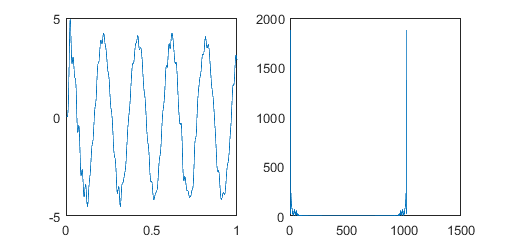
\includegraphics{pictures/filt_sig.png} \\ Рис.5 Сигнал после фильтрации

Создадим схему в Simulink
\center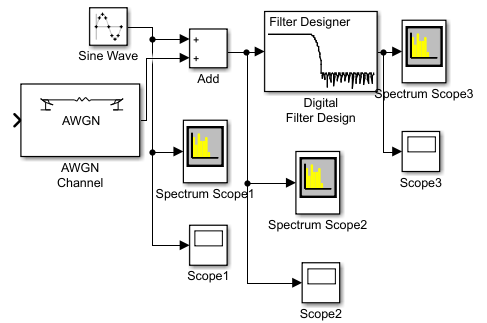
\includegraphics{pictures/simul.png} \\ Рис.7 Схема

Сгенерируем гармонический сигнал в Simulink
\center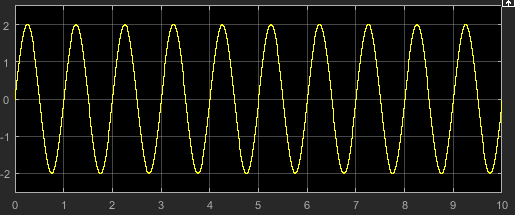
\includegraphics{pictures/SimulSignal.png} \\ Рис.8 Сигнал
\center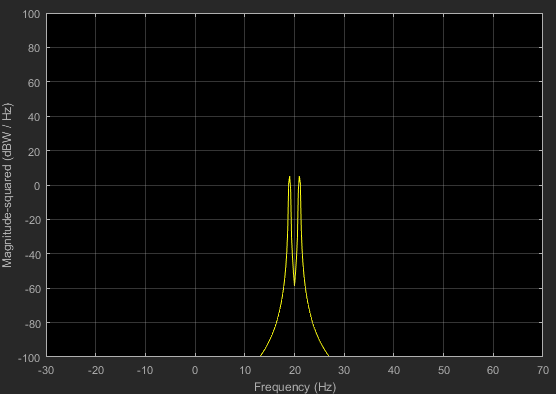
\includegraphics{pictures/SimulSpecSignal.png} \\ Рис.9 Спектр сигнала

Добавим к нему шум
\center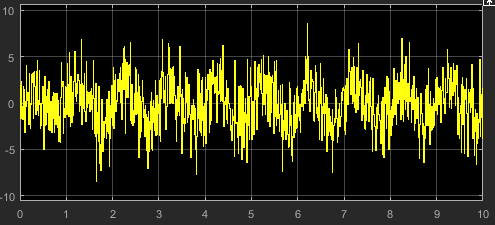
\includegraphics{pictures/SimulShum.png} \\ Рис.10 Зашумленный сигнал
\center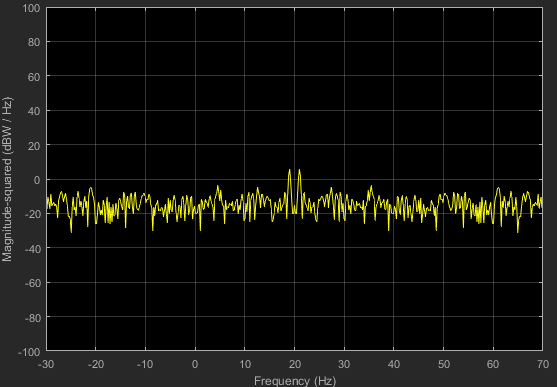
\includegraphics{pictures/SimulSpecShum.png} \\ Рис.11 Спектр зашумленного сигнала


Выполним фильтрацию сигнала
\center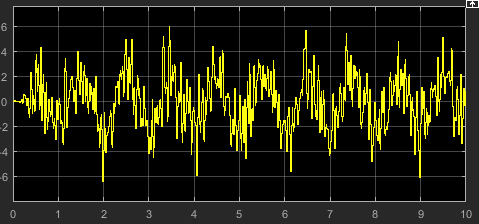
\includegraphics{pictures/SimulFiltSig.png} \\ Рис.12 Сигнал после фильтрации
\center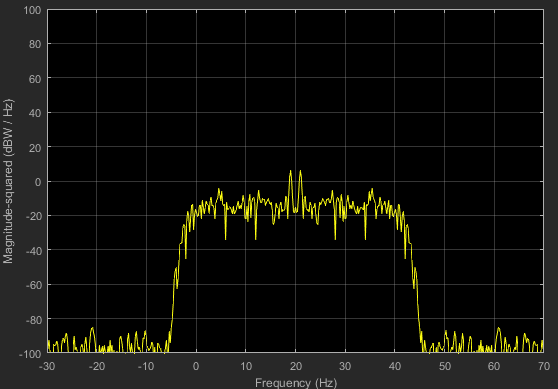
\includegraphics{pictures/SimulSpecFiltSig.png} \\ Рис.13 Спектр сигнала после фильтрации



\section{Вывод}
В ходе выполнения лабораторной работы мы познакомились с ФНЧ и применили его на тестовый сигнал с шумом. Был создан сигнал, зашумлен и отфильтрован как в Matlab, так и в Simulink. Видно, что действительно ФНЧ отфильтровал сигнал, но он не полностью совпадает с исходным. Это объясняется тем, что часть шума имеет низкие частоты, которые фильтр не может подавить и именно этот шум искажает наш сигнал.


\end{document}
